\documentclass[12pt]{article}

\usepackage[margin=1in]{geometry}
\usepackage{amsmath}
\usepackage{amssymb}
\usepackage{graphicx}
\usepackage{hyperref}
\usepackage{setspace}
\usepackage{titlesec}
\usepackage{booktabs}
\usepackage{enumitem}
\usepackage{parskip}
\usepackage{fancyhdr}
\usepackage{array}
\usepackage[numbers]{natbib}
\usepackage{float}

\hypersetup{
    colorlinks=true,
    linkcolor=black,
    urlcolor=blue,
    citecolor=black
}

\pagestyle{fancy}
\fancyhf{}
\rhead{CSDS 395}
\lhead{SkillSync}
\rfoot{\thepage}

\titleformat{\section}{\large\bfseries}{\thesection.}{0.5em}{}
\titleformat{\subsection}{\normalsize\bfseries}{\thesubsection}{0.5em}{}

\begin{document}

\begin{titlepage}
    \centering
    \vspace*{1cm}
    
\includegraphics[width=0.35\textwidth]{black_cw.png}\\[1.5cm]
    {\Large\bfseries Senior Project In Computer Science\\[0.4em]
    Final Report\\[0.4em]
    }
    \vspace{2cm}
    {\Huge\bfseries SkillSync\par}
    \vspace{2cm}
    {\large
    Jack Alberto (jia15)\\
    Tommaso Beretta (txb341)\\
    William Hugus (wmh42)\\
    Maximilian Schulten (mls384)\\
    Nathaniel Hahn (nrh51)\par}
    \vfill
    {\large April 22, 2026\par}
\end{titlepage}

\tableofcontents
\newpage

\section{Project Summary}

SkillSync is a web app that matches a user with online job listings based on an uploaded PDF of their resume. 
While done before, we aim to provide a lightweight portable solution that does not record data or store data from user uploads while still providing a worthwhile service.

\section{Background \& Related Work}

\subsection{Background}

Traditionally, job searching can be a long and inefficient process. It relies on personal judgment to measure fit with the job before applying. 
SkillSync will provide the user with a data-driven recommendation on job openings that match their skill set and experience. 
There will be no more guessing or hoping that a person's skill set is the right fit for the job. Employers in industry have access to tools such as Applicant Tracking System (ATS) to parse and analyze resumes quickly, while those looking for employment do not have these same tools available to them. SkillSync provides a solution to this inefficiency that many around the world experience.

Solutions like this have been done before, though they are often behind a subscription service, require the user to give personal info, or track the user's personal information. This project will attempt to extract the positive effects that this framework can provide, while minimizing the downsides that often come with the solutions available today.

\subsection{Related Work}

Several papers have recently been published showing strong performance with machine learning or AI models that match resumes to job descriptions. These works use similar but different strategies to output a match score given a resume and a job description. We will use this research to build our lightweight model efficiently scoring resume/job matches.

\begin{itemize}[leftmargin=1.5em]
    \item \textbf{Smart-Hiring: An Explainable End-to-End Pipeline for CV Information Extraction and Job Matching} \cite{smarthiring2025} (2025)
    \begin{itemize}
        \item Uses end-to-end natural language processing (NLP) to extract shared information between a job description and a resume
        \item Encodes both the resume and description in a shared vector space and calculates similarity metrics
    \end{itemize}

    \item \textbf{AI-driven semantic similarity-based job matching framework for recruitment systems} \cite{aidriven2026} (2026)
    \begin{itemize}
        \item Leverages NLP techniques, specifically TF-IDF vectorization and cosine similarity scoring, with domain-specific keyword weighting
        \item Interprets conceptual relevance between resumes and job descriptions, enabling more accurate and inclusive recruitment outcomes
        \item These methods are more effective than basic keyword matching
    \end{itemize}

    \item \textbf{Skills prediction based on multi-label resume classification using CNN with model predictions explanation} \cite{cnn2020} (2020)
    \begin{itemize}
        \item Uses CNN architecture for skill extraction from resumes with strong results
        \item Multi-layer classification: multiple outputs for each resume yielding a set of skills
    \end{itemize}

    \item \textbf{GLiNER: Generalist Model for Named Entity Recognition using Bidirectional Transformer} \cite{gliner2023} (2023)
    \begin{itemize}
        \item Employs embeddings created by a BERT-style encoder-only bidirectional transformer
        \item Performs zero-shot named entity recognition on arbitrary entity labels
        \item Outperforms LLMs on NER benchmarks
    \end{itemize}
\end{itemize}

\section{Project Requirements and Specifications}

SkillSync should provide users with a minimalistic experience while promoting proper UI/UX principles to ensure ease of use, creating a worthwhile output that improves users' job search experience.

\subsection{Requirements}

\textbf{Functional and Effective UI}

The UI must:
\begin{itemize}
    \item Include a place for resume uploads, and handle text extraction from resumes in the browser to free server resources. SkillSync will allow PDFs and Word documents.
    \item Display job matches in a consistent style with hotlinks to the postings for easy navigation by the user.
    \item Display rationale around matches, i.e., skills recognized (or not recognized) and an interpretable scoring breakdown of all three axes.
    \item Appear professional and instill confidence in the results provided to users.
\end{itemize}

\textbf{Resume Matching}

In order to match users with jobs effectively, SkillSync must:
\begin{itemize}
    \item Extract relevant information from the plain text of a user's resume.
    \item Given a job, determine whether a user is a good match based on their resume.
\end{itemize}

\textbf{Security and Privacy}

Frontend and backend will follow industry standards for data privacy and security:
\begin{itemize}
    \item Removal of direct identifiers (name, email, phone number, address).
    \item HTTPS/TLS for data in transit.
\end{itemize}

\subsection{Code Constraints}

\begin{itemize}
    \item All front-end code will be written in HTML, CSS, and JavaScript.
    \item All backend code will be written in Python.
    \item Flask will serve as the connectivity layer between the frontend and backend.
    \item The code must be testable and robust against edge cases.
    \item The final app will be containerized using Docker to ensure portability.
\end{itemize}

\subsection{Design Specifications Met}

All requirements and specifications described in Sections~3.1 and 3.2 are met completely except for the implementation of HTTPS and TLS, because the project has not been deployed.
The project currently runs via Uvicorn, a WSGI server, and is containerized through Docker.

\section{System Outline and Architecture}

\subsection{System Outline}

SkillSync is divided into four main steps:

\begin{enumerate}
    \item \textbf{Skill Extraction:} The user uploads a resume, skills are extracted, and personally identifiable information is removed.
    \item \textbf{Job Aggregation:} Multiple APIs are queried to maximize job opportunities. Each job has key features extracted.
    \item \textbf{Scoring:} The skills extracted in step one are matched with the job features extracted in step two, and considered in the scoring algorithm alongside education and semantic scores.
    \item \textbf{Match Presentation:} The ordered top matches are presented to the user in a clean and functional UI after complete analysis.
\end{enumerate}

\subsection{System Architecture}

SkillSync is built as a three-tier web application. The front end is a single-page interface where users paste their resume and receive a ranked list of job matches.
It communicates with a Flask backend that exposes two REST endpoints: \texttt{/findjobs} for full pipeline execution and \texttt{/score-job} for scoring a single listing. 
The back end orchestrates a multi-stage NLP pipeline: resume parsing and classification, job aggregation, skill extraction, and composite scoring. 
All components are containerized via Docker with memory limits set to the resource demands of the embedded transformer models.

\begin{figure}[H]
    \centering
    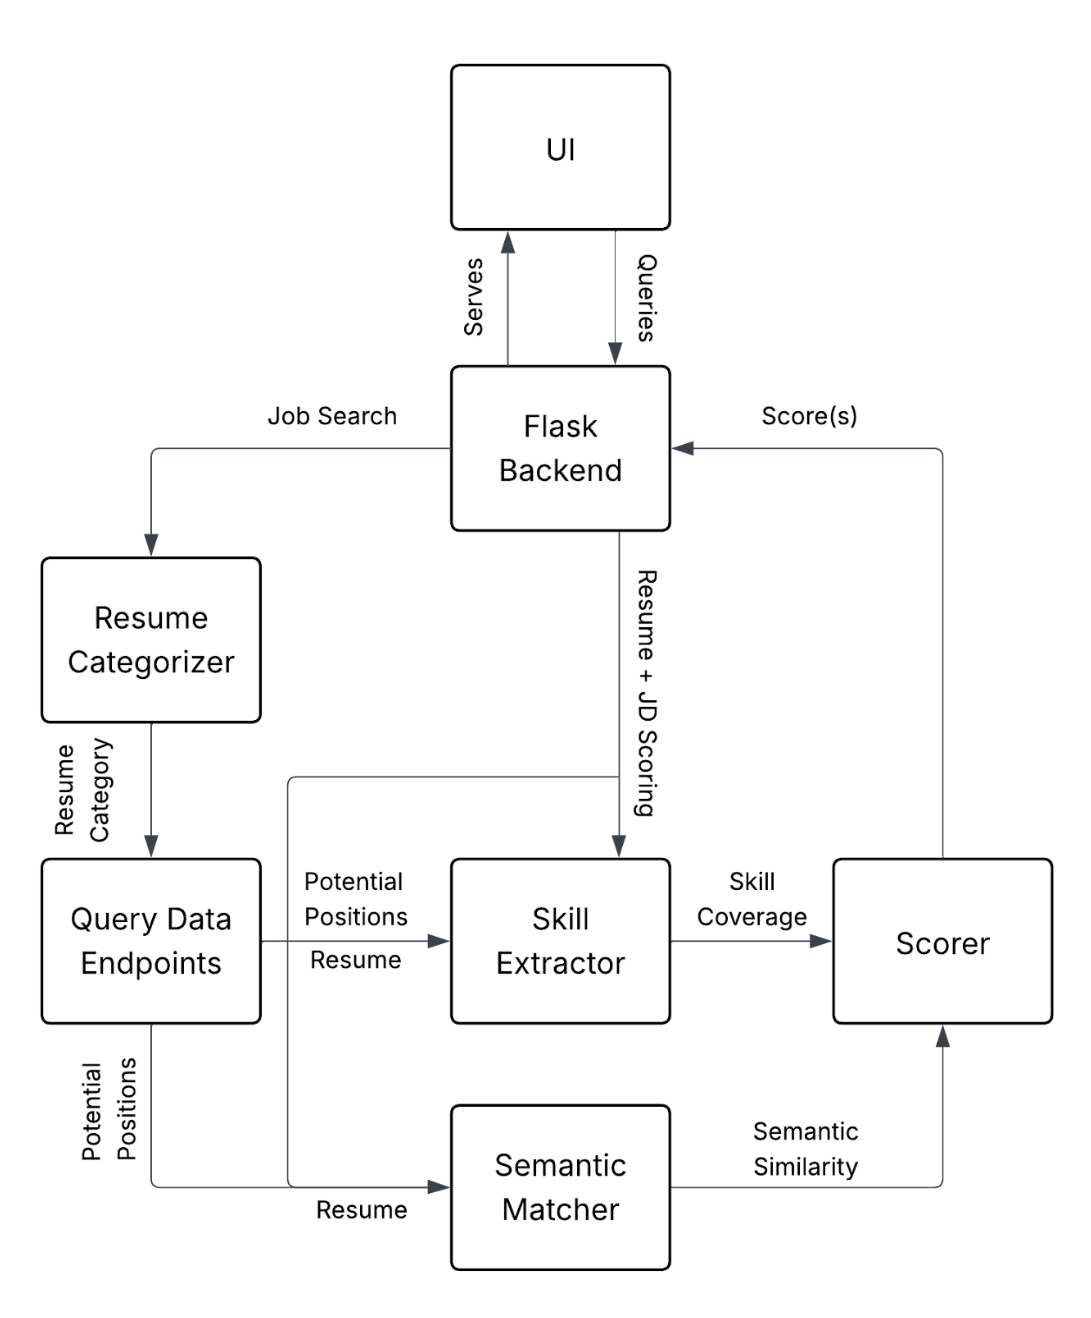
\includegraphics[width=0.85\textwidth]{fig1.png}
    \caption{System Architecture}
    \label{fig:architecture}
\end{figure}

\begin{figure}[H]
    \centering
     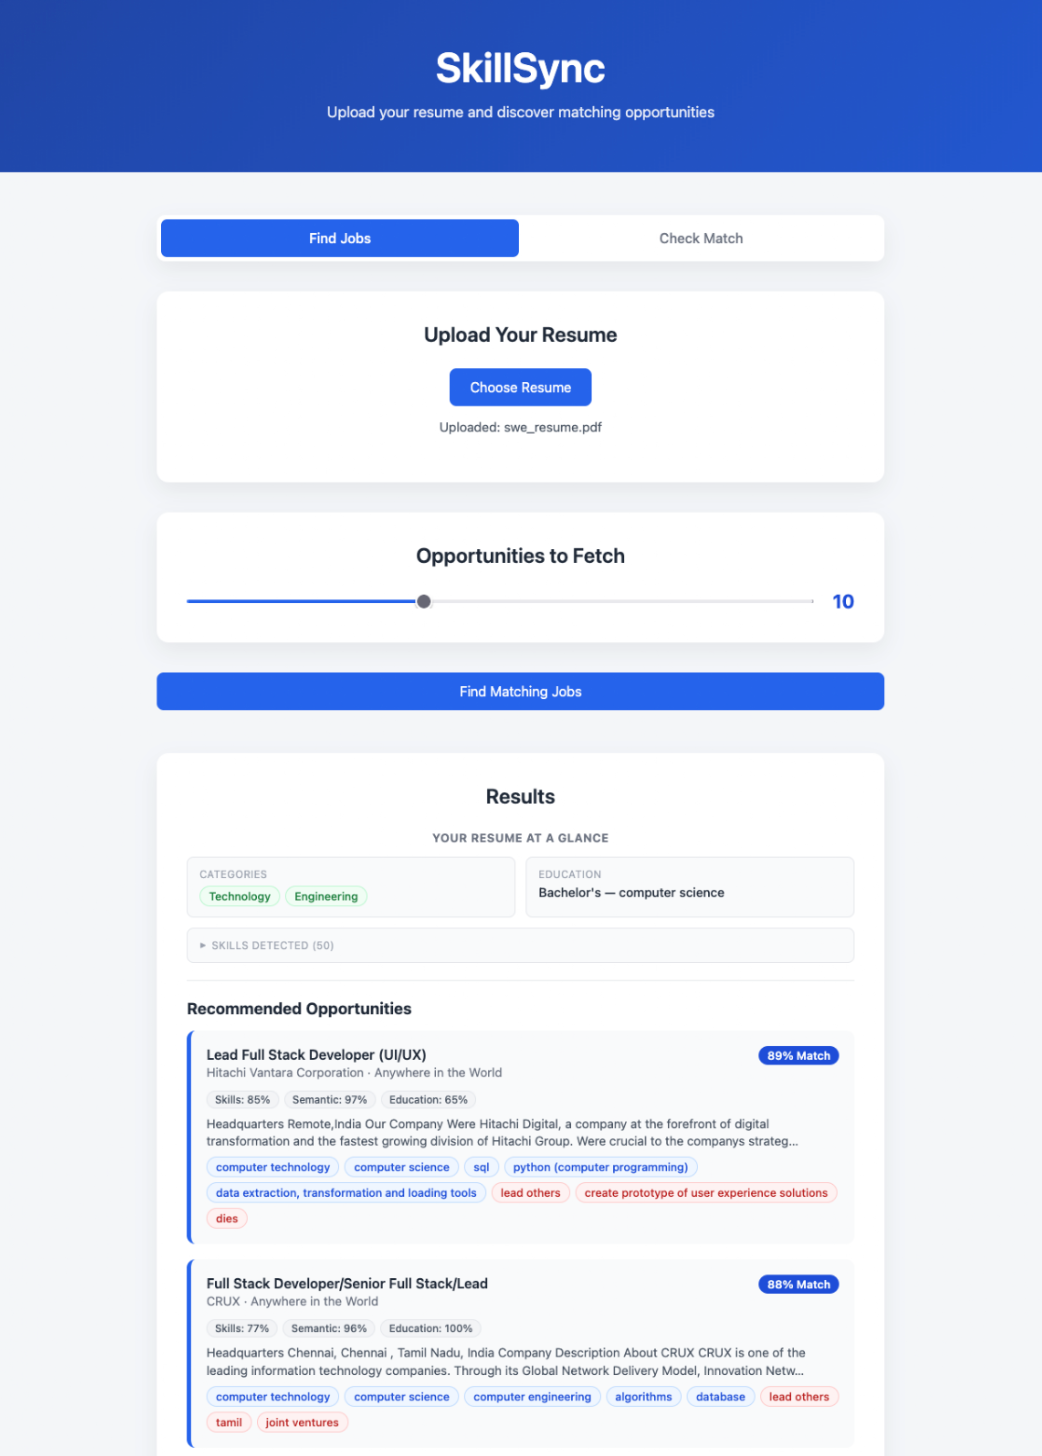
\includegraphics[width=0.85\textwidth]{fig2.png}
    \caption{Front End Example}
    \label{fig:frontend}
\end{figure}

\section{Skill Extraction and Preprocessing}

Before a resume is passed from the frontend to the backend, it is converted in the browser to plain text. 
This step is completed in the browser to keep this workload off of the server. Once the raw resume text is passed to the backend, a thorough cleaning and de-identification process is performed. 
Non-alphanumeric characters are removed and excess whitespace is stripped. Using regex and zero-shot NER via GLiNER, PII obfuscation is performed using general masking tokens (e.g., \texttt{[PERSON]}),
after which the resume is considered cleaned and moves further down the pipeline.

Skills are then extracted using two methods: first, using the European Commission's European Skills, Competences, Qualifications and Occupations (ESCO) database~\cite{esco_ontology}, and second, 
the United States Department of Labor O*NET database~\cite{onet_database}. A JSON file was created containing known skills and some alternative names under which they may be referenced. 
The first pass of the skill extraction deterministically searches the resume for these known skills using spaCy~\cite{spacy}, an NLP library for Python. 
Once exact matches are counted, the second phase of the pipeline incorporates GLiNER, a bidirectional transformer model with roughly 500 million parameters, to perform zero-shot named entity recognition.

The GLiNER model, created by Zaratiana et al.~\cite{gliner2023}, uses a BERT-style transformer model and two parallel feed-forward networks to perform named entity recognition on arbitrary entity labels. 
This enables an effective ``semantically aware'' skill extraction by passing named entity labels such as ``job skill'' and ``technical ability'' alongside the resume text, with a confidence threshold of 0.7.
Skills extracted this way are deduplicated using the skill map and stored. This process occurs for both the resume and the job description, producing a skill list for each that is used for downstream scoring.

\section{Front End}

The interface is minimal and clean, featuring a resume text input and a results panel. 
After submission, users see each job ranked by composite match score, with per-job breakdowns of matched skills, unmatched skill gaps, and sub-scores for skill coverage, semantic similarity, and education alignment. 
This transparency lets users understand why a job ranked highly rather than treating the score as a black box.

The front end is written in vanilla JavaScript, HTML, and CSS to ensure a lightweight and performant interface.
Heavier JavaScript frameworks were foregone due to their frequent bloating of projects with extensive dependencies even for small projects such as this one. 
This design choice keeps the memory footprint of our Docker images manageable, as the backend Python dependencies (such as PyTorch) already grow the image size considerably.

\section{Data Aggregation}

Job opening data was pulled from 8 different sources: USAJobs~\cite{usajobs_api}, Adzuna~\cite{adzuna_api}, Findwork.dev, The Muse~\cite{themuse_api}, We Work Remotely, Jobicy, Himalayas, and Remote.
Data is then normalized into a common job object from its original schema. Jobs are filtered to remove duplicates and incomplete posts, ensuring unique listings.

\begin{figure}[H]
    \centering
    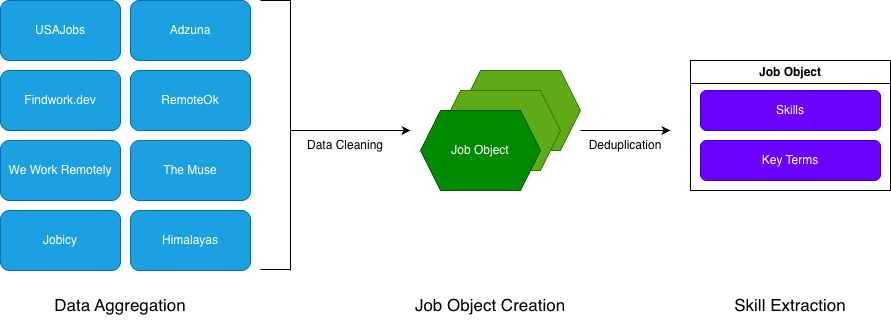
\includegraphics[width=0.85\textwidth]{data_agg.drawio.png}
    \caption{Data Aggregation Pipeline}
    \label{fig:aggregation}
\end{figure}

Before the full matching pipeline is run, two heuristic filters are applied on the returned job descriptions. 
First, the number of exact skill matches between the resume and each job description is counted. Second, regex patterns are used to estimate both the position's seniority and the candidate's seniority.
Jobs whose seniority level is more than one hierarchical rank above the candidate's resume are filtered out. 
The top $k$ results (where $k$ is selected by the user during querying) are then committed through the full scoring pipeline.
We acknowledge the potential limitations of this approach and propose possible solutions in Section~10.

\section{Matching Model}

SkillSync scores each job listing against a parsed resume using a convex combination of three complementary signals:

\begin{equation}
    S_{\text{total}} = \alpha S_{\text{skill}} + \beta S_{\text{sem}} + \gamma S_{\text{edu}}, \quad \alpha + \beta + \gamma = 1
\end{equation}

\noindent\textbf{Default Weights:} $\alpha = \beta = 0.45$, $\gamma = 0.1$

The scoring function is a convex combination of three scoring axes: semantic score, skill coverage, and education coverage. 
Under random resume and job description testing, the resulting distribution was found to be centered below 0.5. 
This is expected: random job and job description pairs are unlikely to be good matches across industries. 
Therefore, the final empirical score distribution is roughly normal with some right skew, centered around 0.4 (see Figure~\ref{fig:score_dist}).
The coefficients $\alpha$, $\beta$, and $\gamma$ were adjusted empirically by evaluating the pipeline on a set of resumes and job descriptions, guided by the intuition that skill and 
experience alignment is a significantly better predictor of match quality than education level alone.

\subsection{Resume Classification}

The matching process starts with resume classification.
Querying all eight API endpoints for every resume was determined to be too computationally heavy.
To narrow the number of results and provide consistently competitive matches, a machine learning classifier~\cite{scikit-learn} was trained on the embeddings of a corpus of roughly 13,000 resume--industry pairs.
The classifier places resumes into two general categories: technology and/or business and management. This allows the program to parameterize API calls to improve the probability of finding strong fits with less data.


\subsection{Skill Coverage ($S_{\text{skill}}$)}

Skill coverage is computed by matching deterministically from databases aggregated from O*NET and ESCO, alongside a fuzzy matching system leveraging \texttt{all-MiniLM-L6-v2} embeddings and cosine similarity:

\begin{equation}
    S_{\text{skill}} = \phi\!\left(\frac{1}{|J|} \sum_{j \in J} w\!\left(\max_{r \in R} \cos(e_j, e_r)\right)\right)
\end{equation}

\noindent where $w(x)$ rewards matches above threshold $\tau = 0.6$, and $\phi$ applies a shifted sigmoid function to ensure saturation at acceptable raw coverage values.

A key challenge was that exact  ignores semantically similar matches. 
For example, ``familiar with AWS'' in a resume and ``familiarity with cloud platforms'' in a job description would not return an identical match, yet they are semantically equivalent.
This discrepancy is resolved by computing a dense vector representation of every skill in both the resume and job description via an embedding model, then computing a pairwise similarity matrix. 
Specifically, $w(x)$ operates as a step function: skills with cosine similarities $\geq 0.8$ receive a ``direct'' match score of 1.0; skills in the range $(0.6,\, 0.8)$ receive a ``soft'' match score of 0.6; anything below this threshold is considered a miss and scores 0.

\subsection{Semantic Similarity ($S_{\text{sem}}$)}

To capture contextual alignment beyond discrete skills, the resume and job description are each segmented into overlapping windows of 30 tokens with stride 10.
The mean of per-window maximum cosine similarities $\bar{s}$ is mapped to a calibrated score via a normal CDF fit empirically to 25,000+ job--resume pairs ($\mu = 0.345$, $\sigma = 0.067$):

\begin{equation}
    S_{\text{sem}} = \Phi_{\mu,\sigma}(\bar{s}), \quad \bar{s} = \frac{1}{|W_J|} \sum_{w \in W_J} \max_{v \in W_R} \cos(e_w, e_v)
\end{equation}

This scoring axis acts as a proxy for relevant experience match between a candidate and a job's responsibilities.
Reliable extraction of experience sections from resumes proved difficult due to the variety of resume formats and the brittleness of regex/deterministic rules. 
The sliding window approach is designed to be a proxy for sentences (as many resumes are bulleted, reliable sentence extraction is difficult). For every ``sentence'' in the job description, the system identifies the best-matching ``sentence'' in the candidate's resume by cosine similarity.
The mean of these scores is the raw semantic score. As shown in Figure~\ref{fig:sem_exp1}, the distribution of these scores is quite normal, and post-processing via the empirically fitted normal CDF maps the narrow distribution onto the expected $[0,1]$ co-domain.

\subsection{Education Coverage ($S_{\text{edu}}$)}

Education coverage combines degree-level alignment and major similarity:

\begin{equation}
    S_{\text{edu}} = 0.7\, S_{\text{deg}} + 0.3\, S_{\text{maj}}
\end{equation}

\noindent where $S_{\text{deg}}$ is a hierarchical score (1.0 if the candidate meets or exceeds the required degree level, 0.5 if one level below, 0.0 otherwise), and $S_{\text{maj}}$ is the cosine similarity between embedded major strings, thresholded at $\tau_{\text{edu}} = 0.6$. 
Education and major information is extracted using GLiNER, which proved robust under testing.

\begin{figure}[H]
    \centering
     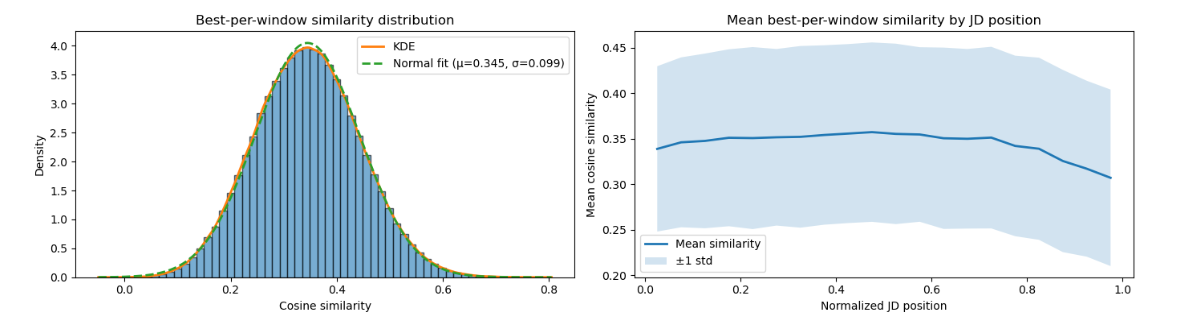
\includegraphics[width=0.85\textwidth]{fig4.png}
    \caption{Semantic Scoring Experiment}
    \label{fig:sem_exp1}
\end{figure}

\begin{figure}[H]
    \centering
    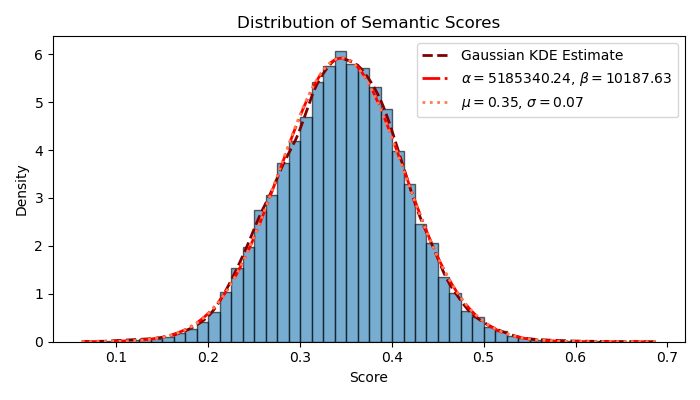
\includegraphics[width=0.75\textwidth]{sem_scores_dist.png}
    \caption{Semantic Scoring Experiment (continued)}
    \label{fig:sem_exp2}
\end{figure}

\section{Testing and Results}

The project features a full \texttt{pytest} suite designed to ensure consistent development among a multi-person team and deployment verification. 
These tests provide coverage across the build, preprocess, extract, and inference modules, allowing verification of changes and bug catching. 
GitHub's continuous integration capabilities via GitHub Actions are employed to automatically test code upon each new push to the main branch.

As mentioned in Section~8, the scoring function is evaluated across 25,000+ randomly paired job description--resume combinations.
The final distribution is roughly normal, and its overall shape confirms that the pipeline discriminates meaningfully rather than saturating at extremes. 
Skill coverage and semantic similarity are positively correlated, validating that both signals capture complementary but consistent notions of fit.
Education alignment shows lower correlation with the other two components, as expected.

\begin{figure}[H]
    \centering
    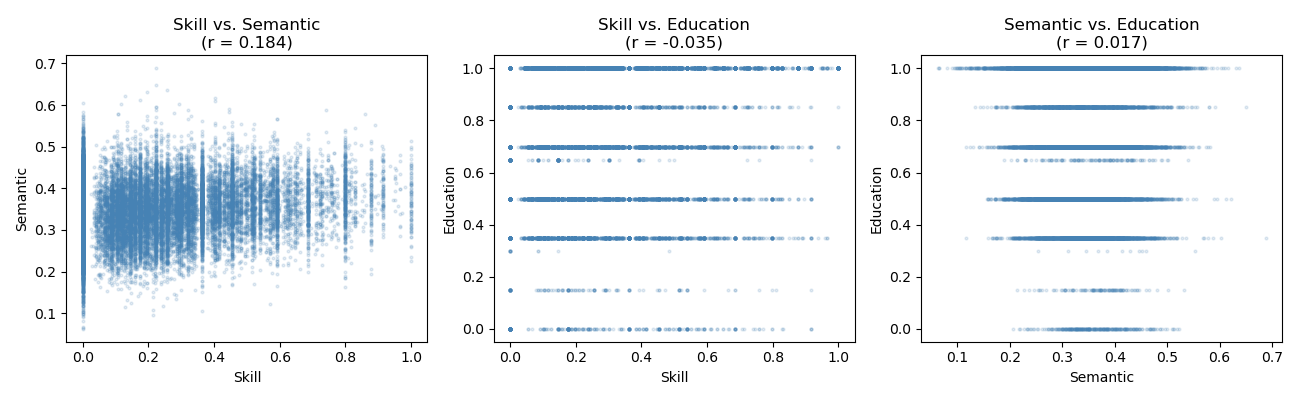
\includegraphics[width=0.85\textwidth]{correlates.png}
    \caption{Scoring Correlates}
    \label{fig:correlates}
\end{figure}

\begin{figure}[H]
    \centering
    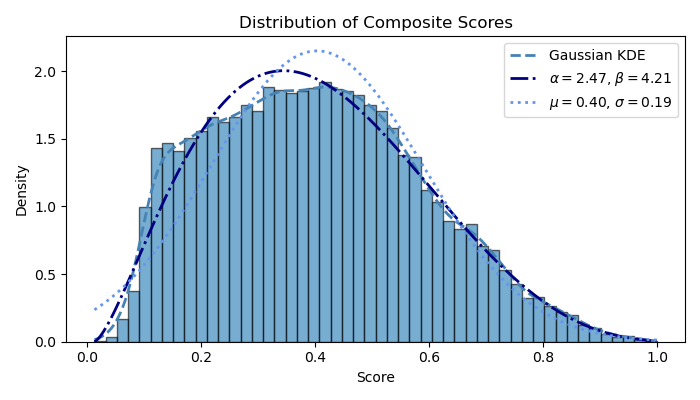
\includegraphics[width=0.75\textwidth]{scores_dist.png}
    \caption{Score Distribution}
    \label{fig:score_dist}
\end{figure}

\section{Conclusion \& Discussion}

The SkillSync project successfully implemented a complete, lightweight, and privacy-focused job matching pipeline. We demonstrated that our approach; which combines deterministic skill database matching, zero-shot NER via GLiNER, and vector-based semantic similarity scoring, creates meaningful separability between strong and poor job matches. Crucially, this high-performance matching framework was achieved without relying on external Large Language Model (LLM) dependencies, which significantly limits server-side computational requirements and cost. This allows SkillSync to offer a valuable, data-driven service with a manageable operational footprint, directly addressing the limitations of many existing, overly complex solutions.

\subsection{Limitations \& Extensions}

While effective, the current SkillSync implementation has several limitations.

First, the reliance on publicly available job descriptions means that boilerplate or highly generic language often present in job postings can confound the semantic similarity signal, potentially over- or under-scoring a candidate's true fit.

Second, the necessary heuristic filtering steps, such as the resume classification in Section~8.1 and the initial job aggregation query parameters, are in place to manage the non-trivial runtime of the full scoring pipeline. Processing over 500 job objects on every user request is computationally unrealistic, but this filtering, while efficient, may inadvertently prevent some highly relevant, niche job matches from ever reaching the candidate.

Potential extensions to this work include:
\begin{itemize}
    \item \textbf{Targeted LLM integration} for specific sub-tasks, such as nuanced skill extraction or generating more detailed match rationales, provided these integrations maintain acceptable latency and cost.
    \item \textbf{Caching} to drastically improve runtime performance. Caching parsed job objects in a secure database would eliminate redundant API calls and processing. Similarly, caching user resumes (post-PII obfuscation) could accelerate subsequent searches, though this would require careful consideration of data governance to maintain privacy commitments.
    \item \textbf{Nightly cache refresh}, querying endpoints and storing relevant jobs in a persistent database, would alleviate some of the need for extensive heuristic filtering and allow more jobs to be considered by the scoring pipeline. Though a plan for preventing stale data from bloating database insatnces would need to be carefully planned and integrated.
\end{itemize}

\bibliographystyle{plainnat}
\begin{thebibliography}{11}

\bibitem{smarthiring2025}
Khelkhal, K. and Lanasri, D.
\newblock Smart-Hiring: An Explainable End-to-End Pipeline for CV Information Extraction and Job Matching.
\newblock \textit{arXiv preprint arXiv:2511.02537}, 2025.
\newblock \url{https://arxiv.org/abs/2511.02537}

\bibitem{aidriven2026}
Ajjam, M.-H. and Al-Raweshidy, H.~S.
\newblock AI-driven semantic similarity-based job matching framework for recruitment systems.
\newblock \textit{Information Sciences}, 724:122728, 2026.
\newblock \url{10.1016/j.ins.2025.122728}

\bibitem{cnn2020}
Jiechieu, K.~F.~F. and Tsopze, N.
\newblock Skills prediction based on multi-label resume classification using CNN with model predictions explanation.
\newblock \textit{Neural Computing and Applications}, 33:5069--5087, 2021.
\newblock \url{10.1007/s00521-020-05302-x}


\bibitem{gliner2023}
Urchade Zaratiana, Nadi Tomeh, Pierre Holat, and Thierry Chanty.
\newblock GLiNER: Generalist Model for Named Entity Recognition using Bidirectional Transformer.
\newblock {\em arXiv preprint arXiv:2311.01090}, 2023.

\bibitem{esco_ontology}
{European Commission}.
\newblock {European Skills, Competences, Qualifications and Occupations (ESCO)}, 2023.
\newblock European Commission DG Employment, Social Affairs and Inclusion.

\bibitem{onet_database}
{U.S. Department of Labor, Employment and Training Administration}.
\newblock {O*NET 28.0 Database}, 2023.
\newblock National Center for O*NET Development.

\bibitem{spacy}
Matthew Honnibal, Ines Montani, Sofie Van~Landeghem, and Adriane Boyd.
\newblock {spaCy: Industrial-strength Natural Language Processing in Python}, 2020.

\bibitem{usajobs_api}
{U.S. Office of Personnel Management}.
\newblock {USAJobs Search API}, 2024.

\bibitem{adzuna_api}
{Adzuna Ltd.}
\newblock {Adzuna Job Search API v1}, 2024.

\bibitem{themuse_api}
{Daily Muse Inc.}
\newblock {The Muse API}, 2024.

\bibitem{scikit-learn}
F.~Pedregosa, G.~Varoquaux, A.~Gramfort, V.~Michel, B.~Thirion, O.~Grisel, M.~Blondel, P.~Prettenhofer, R.~Weiss, V.~Dubourg, J.~Vanderplas, A.~Passos, D.~Cournapeau, M.~Brucher, M.~Perrot, and E.~Duchesnay.
\newblock Scikit-learn: Machine learning in {P}ython.
\newblock {\em Journal of Machine Learning Research}, 12:2825--2830, 2011.

\end{thebibliography}

\end{document}
